\iffalse
\chapter{2009}
\author{AI24BTECH11030}
\section{ae}
\fi

    \item Two vortices of the same strength and sign are placed a distance $d$ apart as shown below. Assume that the vortices are free to move and the fluid is ideal.
    \begin{center}
        
        \begin{tikzpicture}
            
            % Drawing the horizontal line
        \draw[thick] (-3,0) -- (3,0);
        
        % Drawing the two points
        \filldraw (-2,0) circle (2pt) node[below] {1};
        \filldraw (2,0) circle (2pt) node[below] {2};
        
        % Drawing the arrows (torques)
        \draw[->, thick] (-1.75,0.5) arc[start angle=60,end angle=120,radius=0.5] node[pos=0.5,above] {$\Gamma$};
        \draw[->, thick] (2.25,0.5) arc[start angle=60,end angle=120,radius=0.5] node[pos=0.5,above] {$\Gamma$};
        
        % Marking the center point P
        \draw[thick] (0,-0.3) -- (0,0.3);
        \node at (0,-0.5) {$P$};
        
        % Drawing the distance line and marking d
        \draw[<->] (-2,-1) -- (2,-1);
        \node at (0,-1.3) {$d$};
        
    \end{tikzpicture}
    \end{center}
    Which of the following statements is true?  \hfill (GATE AE 2009)
    \begin{enumerate}
        \item Vortices 1 and 2 spiral inwards with an initial angular speed $\frac{\Gamma}{2\pi d^2}$ to finally merge and form one vortex of twice the strength.
        \item Vortices 1 and 2 spiral inwards with an initial angular speed $\frac{\Gamma}{\pi d^2}$ to finally merge and form one vortex of twice the strength.
        \item Vortices 1 and 2 perpetually revolve about the midpoint $P$ with radius of revolution $\frac{d}{2}$ and angular speed $\frac{\Gamma}{2\pi d^2}$.
        \item Vortices 1 and 2 perpetually revolve about the midpoint $P$ with radius of revolution $\frac{d}{2}$ and angular speed $\frac{\Gamma}{\pi d^2}$.
    \end{enumerate}

    \item The laminar boundary layer over a large flat plate held parallel to the flow is $7.2 \, \text{mm}$ thick at a point $0.33 \, \text{m}$ downstream of the leading edge. If the free stream speed is increased by $50\%$, then the new boundary layer thickness at this location will be approximately  \hfill (GATE AE 2009)
    \begin{multicols}{4}
        \begin{enumerate} 
            \item 10.8 mm
            \item 8.8 mm
            \item 5.9 mm
            \item 4.8 mm
        \end{enumerate}
    \end{multicols}

    \item Consider a simply supported beam of length $2L$ with an overhang of length $L$, loaded by an end moment $M$, as shown below. \\
    
    \begin{center}
        \begin{circuitikz}[scale=0.5]
            \tikzstyle{every node}=[font=\LARGE]
            \draw [ line width=1.8pt](6.75,12.5) to[short] (17,12.5);
        \draw [line width=0.9pt, ->, >=Stealth] (16.5,13.5) .. controls (17.5,13) and (17.5,12) .. (16.5,11.5) ;
        \node [font=\normalsize] at (18,12.5) {M};
        \node [font=\normalsize] at (14.5,12) {L};
        \node [font=\normalsize] at (8.75,12) {L};
        \draw [line width=0.2pt, short] (6.75,12.5) -- (6.5,12);
        \draw [line width=0.2pt, short] (6.75,12.5) -- (7,12);
        \draw [line width=0.2pt, short] (6.5,12) -- (7,12);
        \draw [line width=0.2pt, short] (12,12.5) -- (11.75,12);
        \draw [line width=0.2pt, short] (12,12.5) -- (12.25,12);
        \draw [line width=0.2pt, short] (11.75,12) -- (12.25,12);
        % \draw [ line width=0.2pt ] (6.25,12) rectangle (7.25,11.5);
        \draw [ line width=0.2pt ] (11.75,11.75) circle (0.25cm);
        \draw [ line width=0.2pt ] (12.25,11.75) circle (0.25cm);
        % \draw [ line width=0.2pt ] (11.25,11.5) rectangle (12.75,11);
        \draw [line width=0.2pt, short] (6.25,12) -- (6.75,11.5);
        \draw [line width=0.2pt, short] (6.5,12) -- (7,11.5);
        \draw [line width=0.2pt, short] (7,12) -- (7.25,11.75);
        \draw [line width=0.2pt, short] (11.25,11.5) -- (11.75,11);
        \draw [line width=0.2pt, short] (11.75,11.5) -- (12.25,11);
        \draw [line width=0.2pt, short] (12.25,11.5) -- (12.75,11);
        \draw [line width=0.2pt, short] (6.75,12) -- (7.25,11.5);
        \draw [line width=0.2pt, short] (6.25,11.75) -- (6.5,11.5);
        \draw [line width=0.2pt, short] (11.5,11.5) -- (12,11);
        \draw [line width=0.2pt, short] (11.25,11.25) -- (11.5,11);
        \draw [line width=0.2pt, short] (12,11.5) -- (12.5,11);
        \draw [line width=0.2pt, short] (12.5,11.5) -- (12.75,11.25);
        \end{circuitikz}
    \end{center}

    The bending moment distribution for this beam is  \hfill (GATE AE 2009)
    \begin{multicols}{2}
        \begin{enumerate}
            \item
                \begin{minipage}[c]{0.9\linewidth}
                \centering
                \begin{circuitikz}[scale=0.5]
                \tikzstyle{every node}=[font=\LARGE]
                \draw [line width=0.2pt, short] (6.5,12.25) -- (14,12.25);
                \draw [line width=1.4pt, short] (6.5,12.25) -- (10.5,11.5);
                \draw [line width=1.4pt, short] (10.5,11.5) -- (14,13.25);
                \draw [line width=1.4pt, short] (14,13.25) -- (14,12.25);
                \end{circuitikz}
                \end{minipage}\\\\
                
            \item 
                \begin{minipage}[c]{0.9\linewidth}
                \centering
                \begin{circuitikz}[scale=0.5]
                \tikzstyle{every node}=[font=\LARGE]
                \draw [line width=0.2pt, short] (6.5,12.25) -- (14,12.25);
                \draw [line width=1.4pt, short] (6.5,12.25) -- (10.5,11.25);
                \draw [line width=1.4pt, short] (10.5,11.25) -- (14,11.25);
                \draw [line width=1.4pt, short] (14,12.25) -- (14,11.25);
                \end{circuitikz}
                \end{minipage}\\\\
                
            \item 
                \begin{minipage}[c]{0.9\linewidth}
                \centering
                \begin{circuitikz}[scale=0.5]
                \tikzstyle{every node}=[font=\LARGE]
                \draw [line width=0.2pt, short] (7.25,11.25) -- (15.25,11.25);
                \draw [line width=1.4pt, short] (7.25,11.25) -- (7.25,12.25);
                \draw [line width=1.4pt, short] (7.25,12.25) -- (11.25,12.25);
                \draw [line width=1.4pt, short] (11.25,12.25) -- (15.25,11.25);
                \end{circuitikz}
                \end{minipage}\\\\
                
            \item 
                \begin{minipage}[c]{0.9\linewidth}
                \centering
                \begin{circuitikz}[scale=0.5]
                \tikzstyle{every node}=[font=\LARGE]
                \draw [line width=0.2pt, short] (7.25,11.25) -- (15.25,11.25);
                \draw [line width=1.4pt, short] (7.25,11.25) -- (7.25,12.25);
                \draw [line width=1.4pt, short] (7.25,12.25) -- (11.25,10.25);
                \draw [line width=1.4pt, short] (11.25,10.25) -- (11.25,11.25);
                \draw [line width=1.4pt, short] (11.25,11.25) -- (15.25,11.25);
                \end{circuitikz}
                \end{minipage}\\\\
        \end{enumerate}
    \end{multicols}

    \item {For the spring-mass system shown below, the natural frequencies are  \hfill (GATE AE 2009)\\
        \begin{center}
            \begin{circuitikz}[scale=0.5]
                \tikzstyle{every node}=[font=\normalsize]
                \draw [ line width=0.2pt ] (5.25,12.75) rectangle (7.75,11.75);
                \draw [ line width=0.2pt ] (11,12.75) rectangle (13.5,11.75);
                \draw [ line width=0.2pt](7.75,12.25) to[R] (11,12.25);
                \node [font=\normalsize] at (9.375,13.25) {k};
                \node [font=\normalsize] at (6.5,12.25) {$m_1$};
                \node [font=\normalsize] at (12.25,12.25) {$m_2$};
            \end{circuitikz}
        \end{center}

    \begin{multicols}{2}
        \begin{enumerate}
            \item $0$ and $\sqrt{\frac{k(m_1+m_2)}{m_1 m_2}}$
            \item $0$ and $\sqrt{\frac{k(m_1+m_2)}{2 m_1 m_2}}$
            \item $0$ and $\sqrt{\frac{k}{(m_1+m_2)}}$
            \item $0$ and $\sqrt{\frac{k}{2(m_1+m_2)}}$
        \end{enumerate}
    \end{multicols}
    }

    \item The buckling load for a simply supported column of rectangular cross section of dimensions $1 \, \text{cm} \times 1.5 \, \text{cm}$ and length $0.5 \, \text{m}$ made of steel ($E = 210 \times 10^9 \, \text{N/m}^2$) is approximately  \hfill (GATE AE 2009)
    \begin{multicols}{4}
        \begin{enumerate}
            \item 10 kN
            \item 4 kN
            \item 23 kN
            \item 46 kN
        \end{enumerate}
    \end{multicols}

    
    % Q.42
    \item A wing root cross section is idealized using lumped areas (booms) as shown below.
    
    % Diagram for Q42
    \begin{center}
        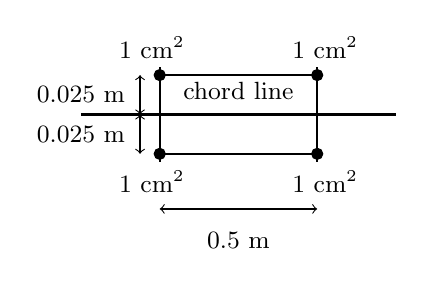
\begin{tikzpicture}
            % Horizontal lines
            \draw[thick] (-2,0) -- (2,0); % chord line
            \draw[thick] (-1,0.5) -- (1,0.5); 
            \draw[thick] (-1,-0.5) -- (1,-0.5); 
            \node at (0, 0.3) {chord line};
            
            % Vertical lines for thickness
            \draw[thick] (-1,0.6) -- (-1,-0.6);
            \draw[thick] (1,0.6) -- (1,-0.6);
            
            % Booms (circles)
            \draw[fill=black] (-1,0.5) circle (2pt);
            \draw[fill=black] (-1,-0.5) circle (2pt);
            \draw[fill=black] (1,0.5) circle (2pt);
            \draw[fill=black] (1,-0.5) circle (2pt);
            
            % Labels
            \node at (-1.1, 0.85) {1 cm$^2$};
            \node at (-1.1, -0.85) {1 cm$^2$};
            \node at (1.1, 0.85) {1 cm$^2$};
            \node at (1.1, -0.85) {1 cm$^2$};
            
            % Dimension labels
            \draw[<->] (-1.25, 0.5) -- (-1.25,0);
            \node at (-2, 0.25) {0.025 m};
            \draw[<->] (-1.25, 0) -- (-1.25,-0.5);
            \node at (-2, -0.25) {0.025 m};
            
            \draw[<->] (-1,-1.2) -- (1,-1.2);
            \node at (0,-1.6) {0.5 m};
        \end{tikzpicture}
    \end{center}
    
    \noindent The wing root bending moment in steady level flight is \( M_y = 10 \, \text{N-m} \). If the airplane flies at a load factor \( n = 3.5 \), the maximum bending stress at the root is:  \hfill (GATE AE 2009)
    \begin{multicols}{4}
        \begin{enumerate}
            \item \( 1 \times 10^6 \, \text{N/m}^2 \)
            \item \( 3.5 \times 10^6 \, \text{N/m}^2 \)
            \item \( 7 \times 10^6 \, \text{N/m}^2 \)
            \item \( 0.286 \times 10^6 \, \text{N/m}^2 \)
        \end{enumerate}
    \end{multicols}
    
    
    % Q.43
    \item A uniform rigid bar of mass \( m = 1 \, \text{kg} \) and length \( L = 1 \, \text{m} \) is pivoted at \( A \). It is supported by a spring of stiffness \( k = 1 \, \text{N/m} \) and a viscous damper of damping constant \( C = 1 \, \text{N-s/m} \), with \( a = \frac{1}{\sqrt{3}} \, \text{m} \) as shown below. The moment of inertia of the rigid bar is \( I_A = \frac{mL^2}{3} \).
    
    
    \begin{center}
        \begin{tikzpicture}
        \tikzstyle{every node}=[font=\small]
        \draw [ line width=0.2pt](8.75,12.75) to[short] (11.25,12.75);
        \draw [ line width=0.2pt](9.25,13.25) to[short] (8.75,12.75);
        \draw [ line width=0.2pt](9.75,13.25) to[short] (9.25,12.75);
        \draw [ line width=0.2pt](10.25,13.25) to[short] (9.75,12.75);
        \draw [ line width=0.2pt](10.75,13.25) to[short] (10.25,12.75);
        \draw [ line width=0.2pt](11.25,13.25) to[short] (10.75,12.75);
        \draw [ line width=0.2pt](11.75,13.25) to[short] (11.25,12.75);
        \draw [ line width=0.2pt](9.5,12.75) to[R] (9.5,10.25);
        \draw [ line width=0.2pt](10.5,12.75) to[short] (10.5,11.75);
        \draw [ line width=0.2pt](10.25,11.75) to[short] (10.75,11.75);
        \draw [ line width=0.2pt](10,12) to[short] (10,11.5);
        \draw [ line width=0.2pt](11,12) to[short] (11,11.5);
        \draw [ line width=0.2pt](10,11.5) to[short] (11,11.5);
        \draw [ line width=0.2pt](10.5,11.5) to[short] (10.5,10.25);
        \draw [ line width=0.2pt ] (10.5,10.25) rectangle (6.5,10);
        \draw [line width=0.2pt, short] (6,10.375) -- (6.5,10.125);
        \draw [line width=0.2pt, short] (6.5,10.125) -- (6,9.875);
        \draw [line width=0.2pt, short] (6,10.375) -- (6,9.875);
        \draw [line width=0.2pt, short] (6,10.75) -- (6,9.75);
        \draw [line width=0.2pt, short] (6,10.75) -- (5.75,10.5);
        \draw [line width=0.2pt, short] (6,10.5) -- (5.75,10.25);
        \draw [line width=0.2pt, short] (6,10.25) -- (5.75,10);
        \draw [line width=0.2pt, short] (6,10) -- (5.75,9.75);
        \draw [line width=0.2pt, short] (6,9.75) -- (5.75,9.5);
        \node [font=\normalsize] at (6.25,10.75) {A};
        \node [font=\small] at (9,11.5) {k};
        \node [font=\small] at (11.25,11.75) {C};

        \draw[<->] (6.5, 9.25) -- (10.5,9.25);
        \node at (8.5, 9) {L};
        \draw[<->] (6.5, 9.75) -- (9.5,9.75);
        \node at (8, 9.5) {a};
        \end{tikzpicture}
    \end{center}
    
    \noindent The system is:  \hfill (GATE AE 2009)
    \begin{enumerate}
        \item Overdamped
        \item Underdamped with natural frequency \( \omega_n = 1 \, \text{rad/s} \)
        \item Critically damped
        \item Underdamped with natural frequency \( \omega_n = 2 \, \text{rad/s} \)
    \end{enumerate}
    
    
    % Q.44
    \item A 2-celled tube with wall thickness 0.5 mm is subjected to a torque of 10 N-m. The resulting shear flows in the two cells are \( q_1 \) and \( q_2 \) as shown below. 
    
    
   \begin{center}
     % Diagram for Q44
     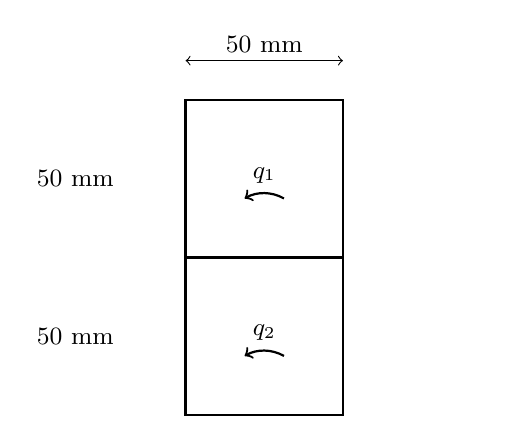
\begin{tikzpicture}
         % Outer rectangle
         \draw[thick] (0,0) rectangle (2,4);
         
         % Middle line
         \draw[thick] (0,2) -- (2,2);
         
         % Labels for shear flows
         \draw[->, thick] (1.25,2.75) arc[start angle=60,end angle=120,radius=0.5] node[pos=0.5,above] {$q_1$};
        %  \node at (1,3) {$q_1$};

        \draw[->, thick] (1.25,0.75) arc[start angle=60,end angle=120,radius=0.5] node[pos=0.5,above] {$q_2$};
        % \node at (1,1) {};
         
         % Dimensions
         \node at (-1.4,3) {50 mm};
         \node at (-1.4,1) {50 mm};
         
         \draw[<->] (0,4.5) -- (2,4.5);
         \node at (1,4.7) {50 mm};
         \node at (3.9,1) {};
     \end{tikzpicture}
   \end{center}
    
    \noindent The torque balance equation (Bredt-Batho formula) for this section leads to:  \hfill (GATE AE 2009)
    \begin{multicols}{2}
        \begin{enumerate}
            \item \( q_1 - q_2 = 2000 \, \text{N/m} \)
            \item \( q_1 + 2q_2 = 2000 \, \text{N/m} \)
            \item \( q_1 + q_2 = 2000 \, \text{N/m} \)
            \item \( 2q_1 + q_2 = 2000 \, \text{N/m} \)
        \end{enumerate}
    \end{multicols}
        

    \item The value of the integral $\int_0^\pi \frac{dx}{1+x+\sin x}$ evaluated using the trapezoidal rule with two equal intervals is approximately  \hfill (GATE AE 2009)
    \begin{multicols}{4}
        \begin{enumerate}
            \item $1.27$
            \item $1.81$
            \item $1.41$
            \item $0.71$
        \end{enumerate}
    \end{multicols}

    \item The product of the eigenvalues of the matrix 
    $
    \myvec{
    2 & 1 & 1 \\
    1 & 3 & 1 \\
    1 & 1 & 4
    }
    $
    is \hfill (GATE AE 2009)
    \begin{multicols}{4}
        \begin{enumerate}
            \item $20$
            \item $24$
            \item $9$
            \item $17$
        \end{enumerate}
    \end{multicols}

    \item In the interval $1 \leq x \leq 2$, the function $f\brak{x} = e^{\pi x} + \sin \pi x$ is  \hfill (GATE AE 2009)
    \begin{multicols}{2}
        \begin{enumerate}
            \item maximum at $x=1$
            \item maximum at $x=2$
            \item maximum at $x=1.5$
            \item monotonically decreasing
        \end{enumerate}
    \end{multicols}

    \item The inverse Laplace transform of $F(s) = \frac{\brak{s+1}}{\brak{s+4}\brak{s-3}}$ is  \hfill (GATE AE 2009)
    \begin{multicols}{4}
        \begin{enumerate}
            \item $\frac{3}{7}e^{4t} + \frac{4}{7}{e^{-3t}}$
            \item $\frac{3}{7}e^{-4t} + \frac{4}{7}e^{3t}$
            \item $\frac{5}{7}e^{-4t} + \frac{6}{7}e^{3t}$
            \item $\frac{5}{7}e^{4t} + \frac{6}{7}{e^{-3t}}$
        \end{enumerate}
    \end{multicols}
